\documentclass{beamer}
\usetheme{Madrid}
\usepackage[utf8]{inputenc}
\usepackage[T1]{fontenc}
\usepackage{graphicx}
\usepackage{lmodern}
\usepackage{movie15}
\usepackage{hyperref}
\usepackage{tikz}
\usepackage{slashbox}

% Pour enlever le \institute du bas de page
% Rapetisser les noms et date etc dans le footer
\setbeamertemplate{footline}
{
      \leavevmode%
      \hbox{%
      \begin{beamercolorbox}[wd=.333333\paperwidth,ht=2.25ex,dp=1ex,center]{author in head/foot}%
      \
      \end{beamercolorbox}%
      \begin{beamercolorbox}[wd=.333333\paperwidth,ht=2.25ex,dp=1ex,center]{title in head/foot}%
      \usebeamerfont{title in head/foot}\insertshorttitle
      \end{beamercolorbox}%
      \begin{beamercolorbox}[wd=.333333\paperwidth,ht=2.25ex,dp=1ex,right]{date in head/foot}%
      \usebeamerfont{date in head/foot}\insertshortdate{}\hspace*{2em}
      \insertframenumber{} / \inserttotalframenumber\hspace*{2ex} 
      \end{beamercolorbox}}%
      \vskip0pt%
}

\AtBeginSection[]
{
      \begin{frame}
            \tableofcontents[currentsection,hideallsubsections]
      \end{frame}
}

\title{Tableau virtuel interactif}
\author{\textcolor{blue}{Baptiste Saleil}, \textcolor{cyan}{Geoffrey Mélia}, \textcolor{blue}{Julien Pagès}, \textcolor{cyan}{Kevin Bollini} \\ \ \\Tuteur de projet: M. Puech}
\date{30 avril 2012}

\begin{document}
	%Kevin
	\begin{frame}
		\titlepage
	\end{frame}

	\section{Introduction}
	\begin{frame}{Introduction}
        
	\begin{block}{But du projet :}
               \begin{itemize}
			\item Lier les compétences AIGLE/IMAGINA
			\item Lier recherches et développement
			\item Concevoir une application incluant une IHM gestuelle
			%\item Fournir des fonctionnalités sociales %Ju et Geo : pas clair du tout
			\item Obtenir des résultats fonctionnels et distribuables
		\end{itemize}
        \end{block}
            
	\end{frame}

      \begin{frame}{Vidéo de présentation}
		% TODO : Tests pour inclure une vidéo : ça marche !
		% \includemovie[poster, text={\small(Exemple d'utilisation)}]{6cm}{6cm}{demo.mp4}
            %\movie{\includegraphics[width=.65\textwidth]{demo}}{demo.ogv}
      \end{frame}

%Plan
      \begin{frame}{Plan}
            \tableofcontents[hideallsubsections]
      \end{frame}
            
      \section{Analyse et Conception}
      \subsection{Choix de conceptions}
            \begin{frame}{Choix de conceptions}
                  \begin{block}{Choix principaux}
                        Découper le projet en deux parties distinctes : \\
                        - une bibliothèque de suivi d'objets réutilisable \\
                        - une application avec une interface naturelle exploitant cette bibliothèque \\
                  \end{block}
            \end{frame}
            
      \subsection{Gestion de projet}
            \begin{frame}{Gestion de projet}
                  \begin{block}{Méthodologie :}
                  \begin{itemize}
                  \item Se renseigner, réaliser une architecture de qualité
                  \item Répartir le travail en fonction des compétences et formations de chacun
                  \item Développer rapidement un prototype
                  \item Développement incrémental en ajoutant des fonctionnalités
                  \end{itemize}
                  \end{block}
            \end{frame}
            
            \begin{frame}{Gestion de projet}
                  \begin{block}{Organisation :}
                  \begin{itemize}
                        \item{Réunions}
                        \item{Deux sous-groupes}
                        \item{Partage des tâches au sein des groupes}
                        \item{Décisions communes (à quatre)}
                  \end{itemize}
                  \end{block}
            
		\begin{block}{Collaboration :}
			\begin{itemize}
			\item{Gestionnaire de versions (Subversion)}
			\item{Partage de documents (Mail et Subversion)}
			\item{Discussions (Mails / Instantanées)}
			\item{Édition collaborative pour le travail à distance (Gobby)}
			\end{itemize}
		\end{block}
            \end{frame}
            
      % Partie de Geoffrey
      \subsection{Analyse}
            \begin{frame}{Analyse}
                  \begin{exampleblock}{Objectifs}
                        \begin{itemize}
                              \item{Identifier les besoins et envies des utilisateurs}
                              \item{Distinguer et classer les fonctionnalités de l'application}
                              \item{Établir un schéma de conception dans le temps}
                              \item{Faciliter le développement, avoir des buts concrets}
                              \item{Produire une application réellement aboutie}
                        \end{itemize}
                  \end{exampleblock}
            \end{frame}
      
      \subsection{Planning}
            \begin{frame}{Rétroplanning}      
                 % Rétroplanning (Diagramme de gantt) :
                  %\begin{center}
                  % TODO : mettre à jour le rétroplanning
                  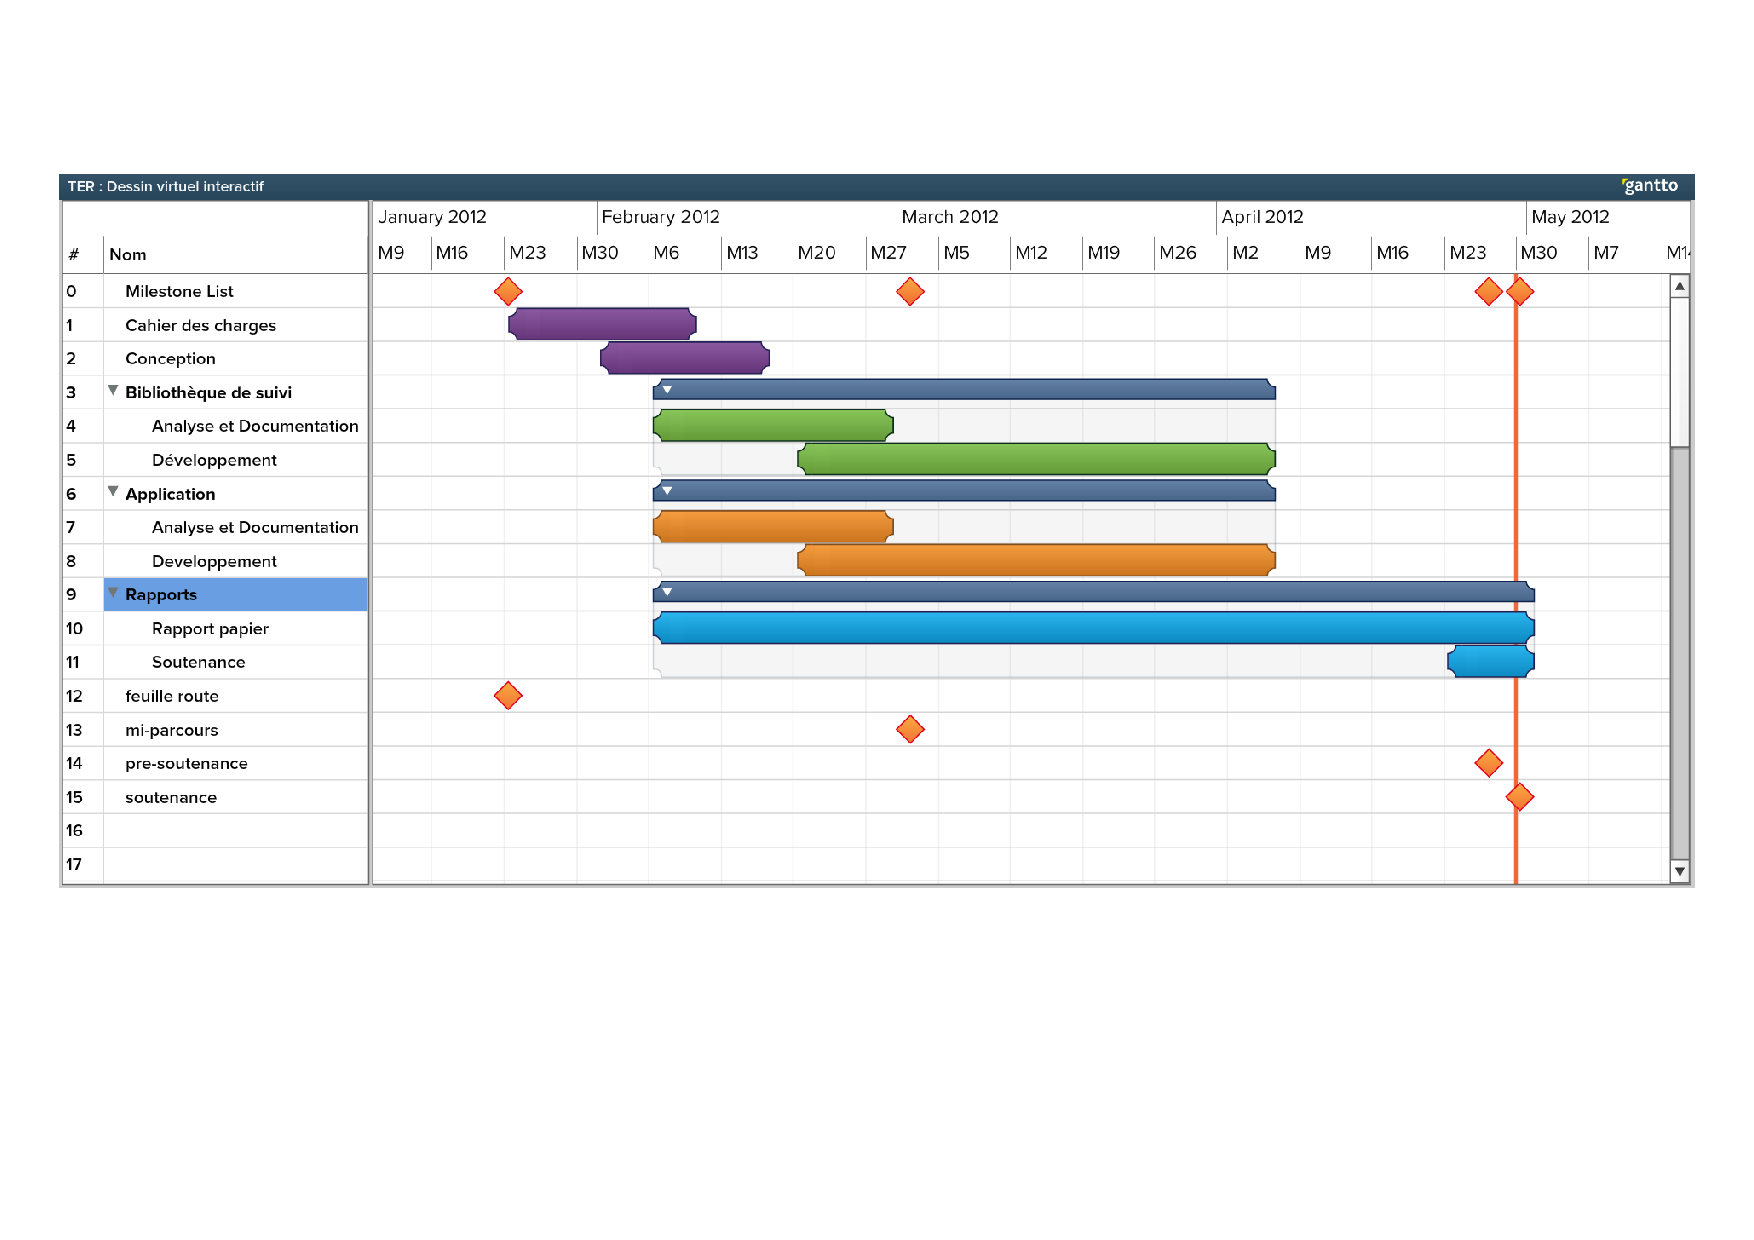
\includegraphics[scale=0.40]{./retro-planning.pdf}
                  %\end{center}
            \end{frame}

      %Partie de Kevin Et Geoffrey
      %Geoffrey
      \section{Bibliothèque}
            \subsection{Architecture}
            \begin{frame}{Bibliothèque de suivi d'objets : libtrack}
                  \begin{block}{Objectifs de la bibliothèque conçue}
                        \begin{itemize}
                        	\item{Utilisation simple sans connaissance en traitement d'image}
                        	\item{Détection d'actions}
                        	\item{Solutions de suivi diverses}
                        	\item{Évaluer et comparer ces solutions}
                        \end{itemize}
                  \end{block}
            \end{frame}

            \begin{frame}{Bibliothèque libtrack}
                  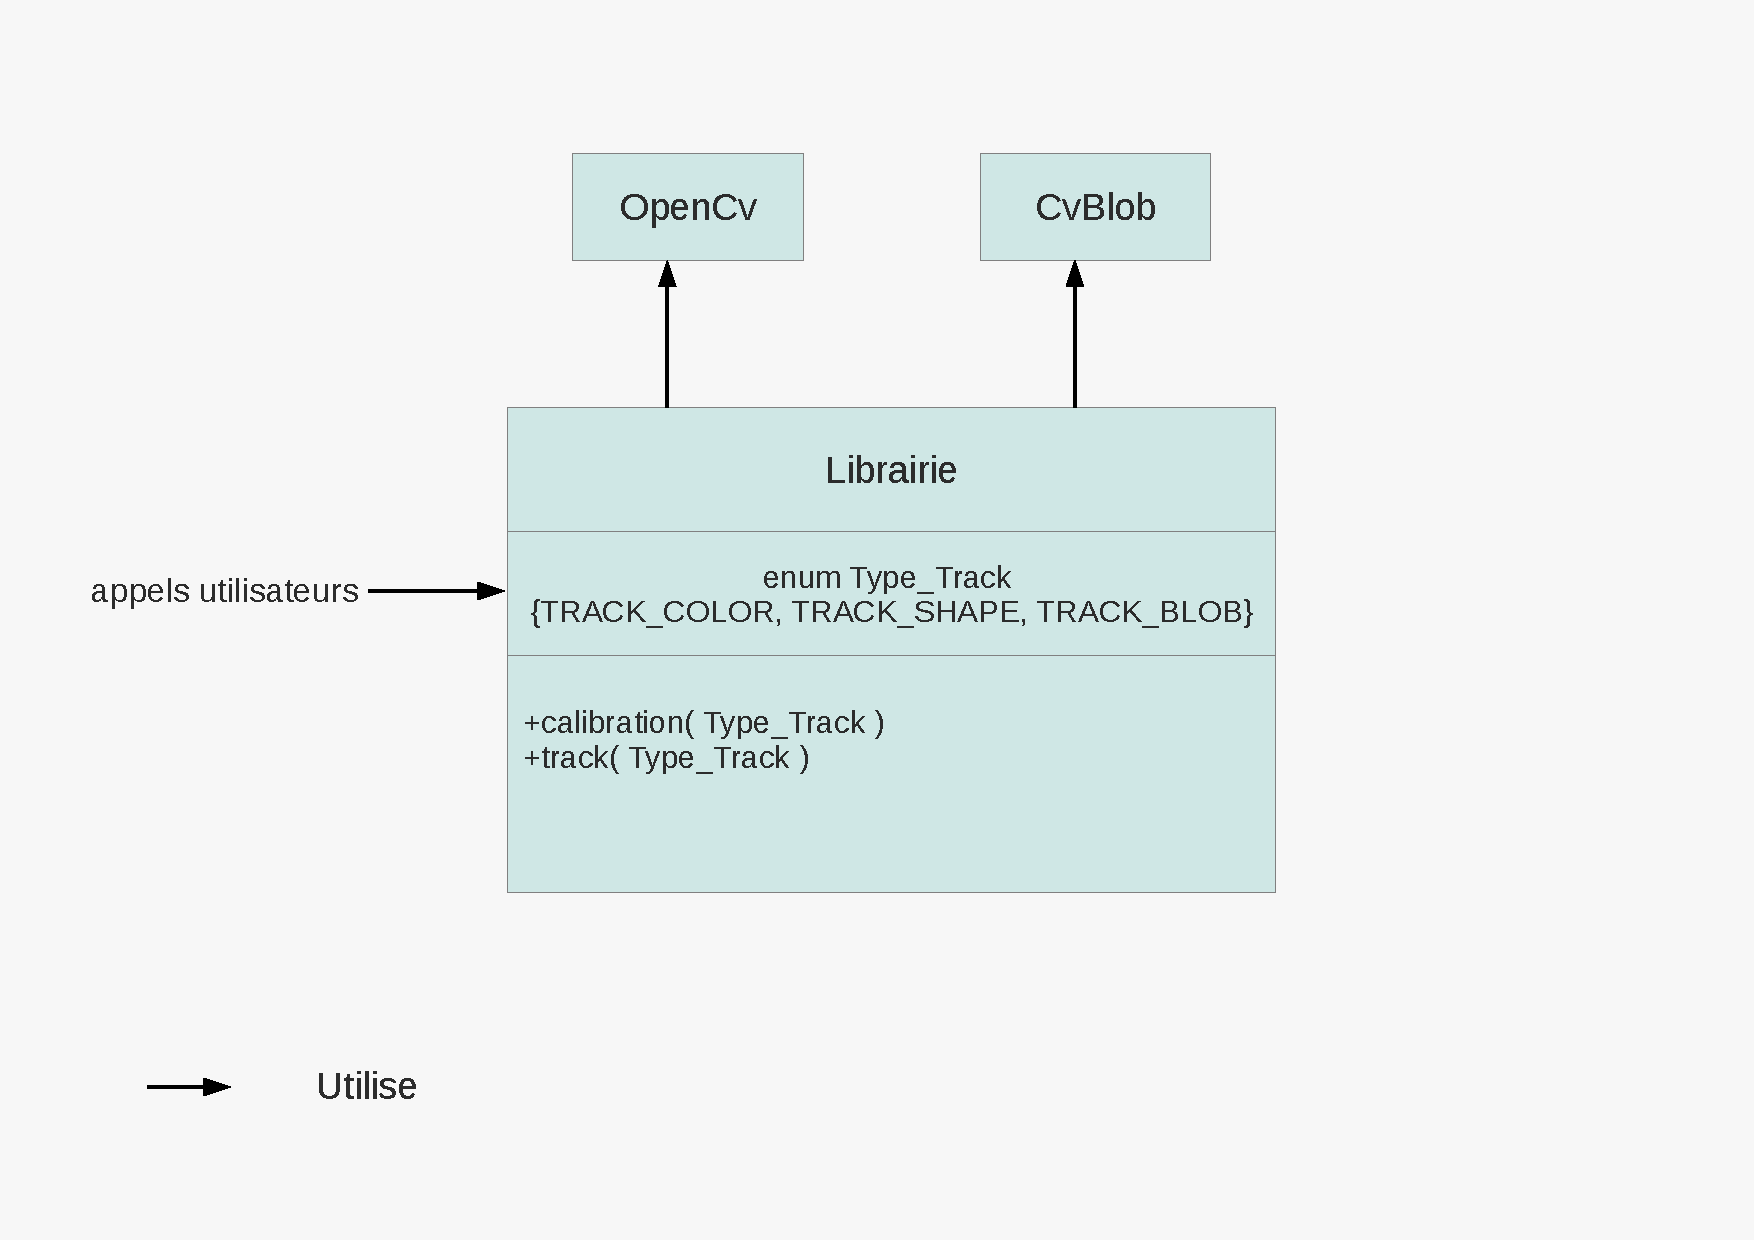
\includegraphics[scale=0.40]{schema-librairie.pdf}
            \end{frame}

            \begin{frame}{Bibliothèque}

            Création d'une structure de données : Cursor\\
	inclure graphique de la structure + énum
            \end{frame}
            
            \begin{frame}{Tableau Comparatif}
		        \begin{table}[h]
				%\begin{center}
				\begin{tabular}{|l|c|c|c|}
				\hline
				\backslashbox{Caractéristique}{Méthode}& Modèle  &C. connexes& Barycentre  \\
				\hline
				Vitesse & -& + & ++ \\
				\hline
				Précision &++&++&+\\
				\hline
				Linéarité &-&+&+\\
				\hline
				Variété curseur &++&+&++\\
				\hline
				Souplesse, adaptation & - - & + &+\\
				\hline
				Sensibilité environnement &++&-&- -\\
				\hline
				Action &Non & Oui & Oui \\
				\hline
				\end{tabular}
				%\end{center}
				\caption{Comparatif des différentes solutions de suivi}
				\label{tableau comparatif}
				\end{table}
			\end{frame}
      %TODO frame a supprimer
            \begin{frame}{Bibliothèque}
            Deux fonctions enveloppes : \\
                  \begin{itemize}
                        \item{Cursor * calibration(IplImage * source, CvPoint A, CvPoint B, TYPE-TRACK flag)}
                        \item{int track(IplImage * source, Cursor * oldCursor)}
                  \end{itemize}            
            \end{frame}

            %Kevin
            \subsection{Fonctionnement}
            \begin{frame}{Scénario type d'utilisation de la bibliothèque}
                  La bibliothèque s'utilise en deux grandes étapes :
                  \begin{itemize}
                        \item{Calibration, engendrant une struture Cursor}
                        \item{Track, mettant à jour les informations de la structure}
                  \end{itemize}
            \end{frame}

            \subsubsection{Calibration}
            \begin{frame}{Calibration : Source d'images et TYPE\_TRACK}
                  \begin{center}
                        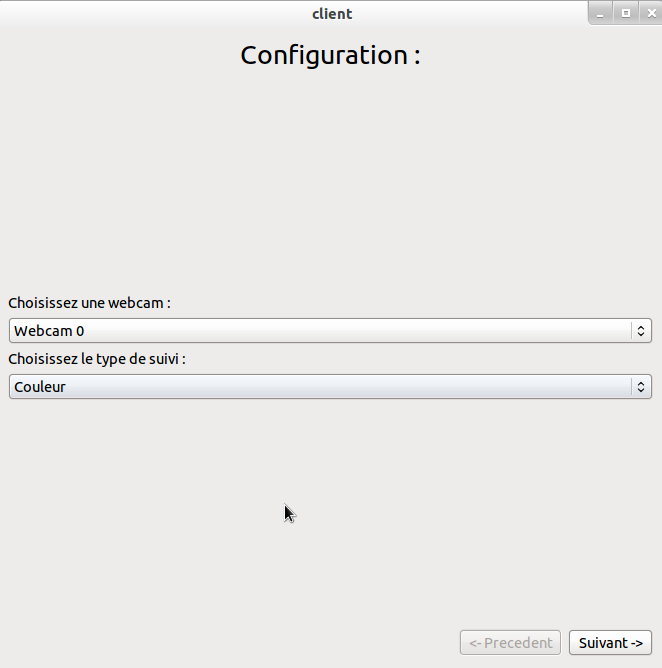
\includegraphics[scale=0.25]{Capture6.png}\\
                        Écran de sélection du Type\_TRACK et de la source d'images
                  \end{center}
            \end{frame}

            \begin{frame}{Calibration : Sélection du curseur}
                  \begin{itemize}
                        \item{Position de l'objet}
                  \end{itemize}
                  \begin{center}
                        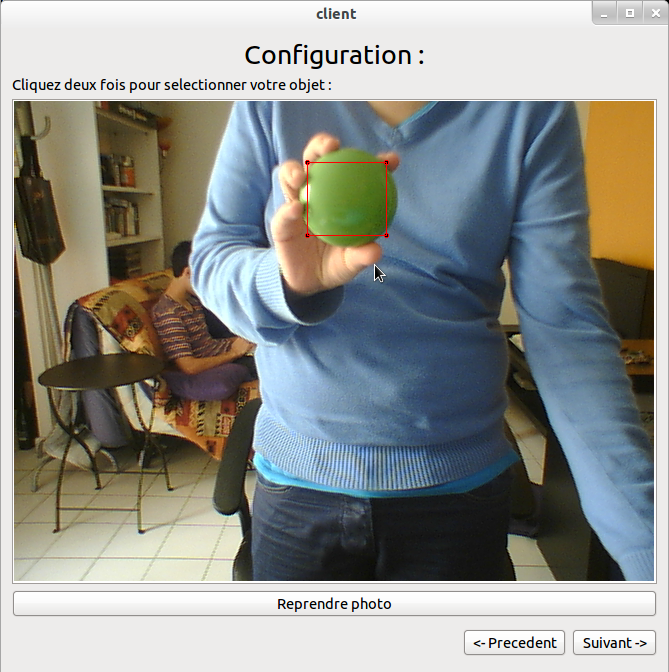
\includegraphics[scale=0.25]{Capture1.png}\\
                        Sélection de l'objet
                  \end{center}
            
            \end{frame}

            \begin{frame}{Calibration couleur : Réglage du seuil}
                  \begin{itemize}
                        \item{Attribut "threshold"}
                  \end{itemize}
                  \begin{center}
                        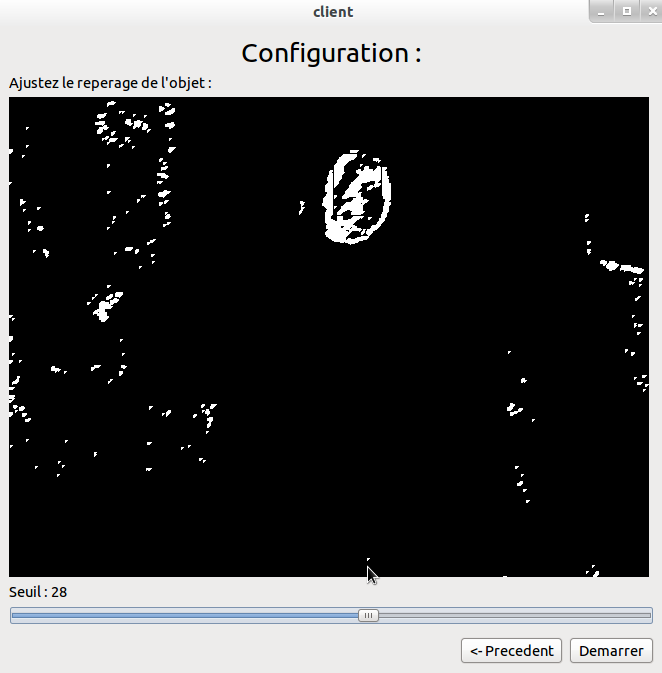
\includegraphics[scale=0.25]{Capture2.png}\\
                        Écran de réglage du seuil
                  \end{center}
            \end{frame}

	    \begin{frame}{Calibration Forme : Extraction du modèle}
                  \begin{itemize}
                        \item{Attribut "mask"}
                  \end{itemize}
                  \begin{center}
                        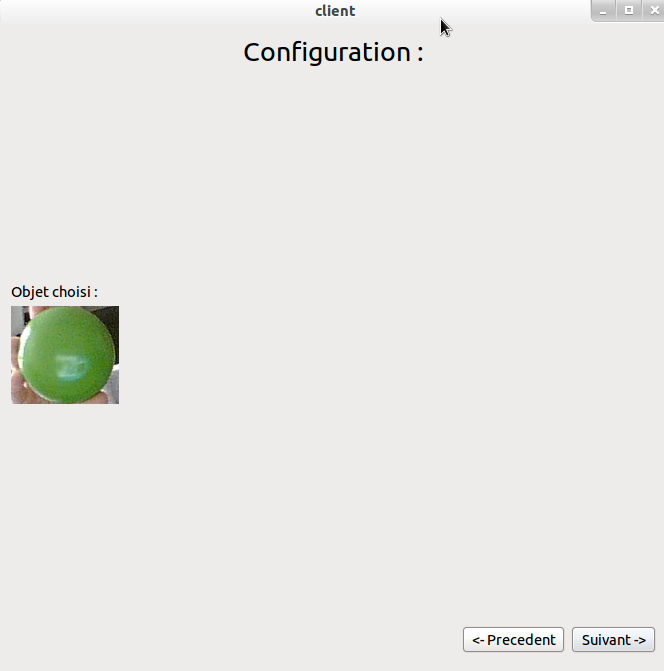
\includegraphics[scale=0.25]{Capture7.png}\\
                        Écran de validation du modèle.
                  \end{center}
            \end{frame}
            
            \subsubsection{Suivi}
            \begin{frame}{Suivi par couleur : Barycentre}
                  \begin{center}
                        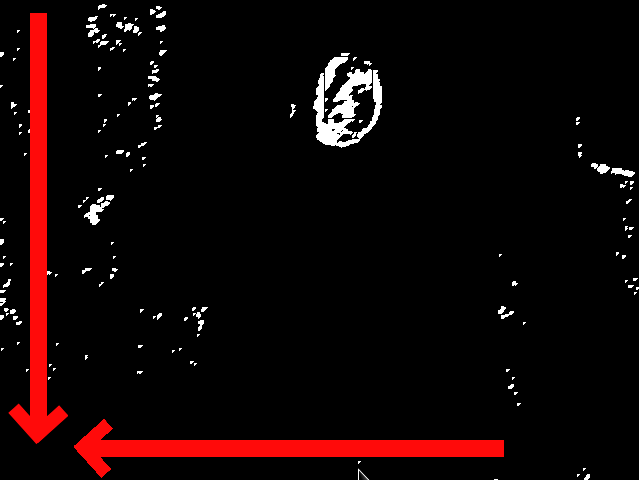
\includegraphics[scale=0.25]{Capture4.png}\\
                        Calcul du barycentre de l'image binaire
                  \end{center}
            \end{frame}

            \begin{frame}{Suivi par Blob : Composantes connexes}
                  \begin{center}
                        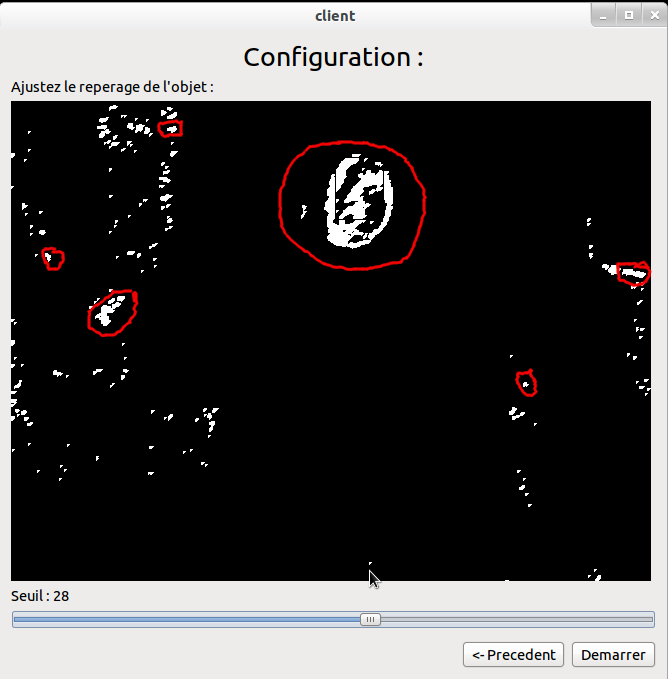
\includegraphics[scale=0.25]{Capture5.png}\\
                        Exploitation des composantes connexes
                  \end{center}
            \end{frame}

            \begin{frame}{Suivi par couleur/Blob : Détection d'action}
                  \begin{itemize}
                        \item{Détection d'action par approchement du curseur}
                  \end{itemize}
                  \begin{center}
                        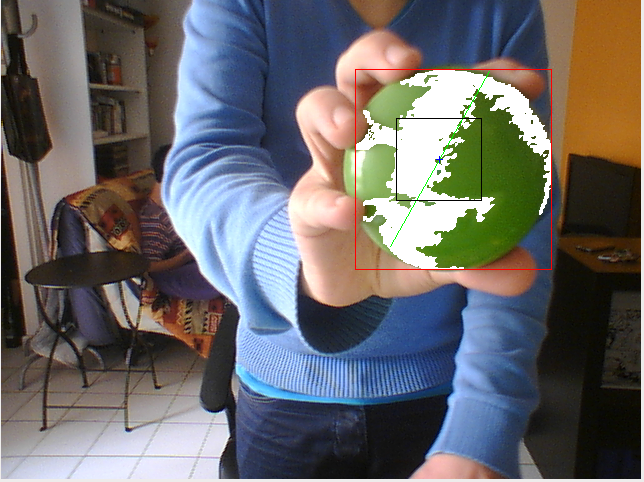
\includegraphics[scale=0.25]{Capture3.png}\\
                        Retour image de l'objet suivi
                  \end{center}
            \end{frame}
            
            %Kevin
            \begin{frame}{Suivi par modèle}
                  \begin{itemize}
                        \item{Recherche du template dans l'image}
                  \end{itemize}
		  \begin{center}
                        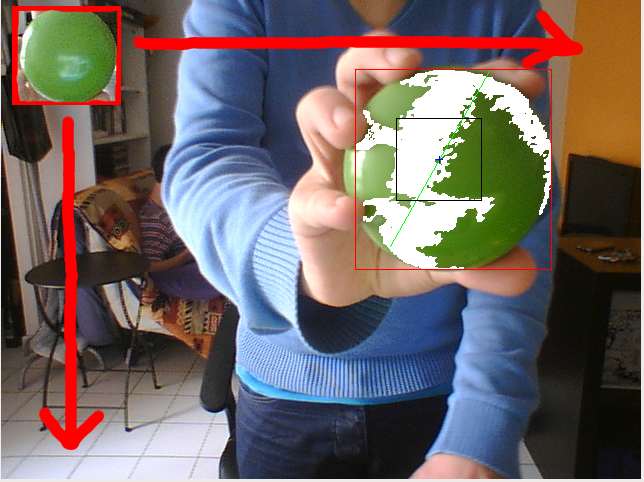
\includegraphics[scale=0.25]{Capture8.png}\\
                        Recherche de modèle.
                  \end{center}
            \end{frame}
            

            \begin{frame}{Résultats}
                  \begin{exampleblock}{Objectifs atteints}
                        \begin{itemize}
                        \item Bibliothèque fonctionelle
                        \item Détection d'actions
                        \item Simplicité d'utilisation
                        \end{itemize}
                  \end{exampleblock}
                  \pause
                  \begin{alertblock}{Difficultés}
                        \begin{itemize}
                        \item Bibliothèques OpenCv/CvBlob
                        \item Détection d'action par modèle
                        \end{itemize}
                  \end{alertblock}
                  \pause		  
                  \begin{block}{Ouverture}
			 \begin{itemize}
                        \item Diversifier
                        \item Optimiser
			\end{itemize}
                  \end{block}				  
            \end{frame}
      
 	% Baptiste et Julien
	% Baptiste
	
	\section{Application}
	
		\subsection{Objectifs}
		\begin{frame}{Objectifs}
			\begin{itemize}
				\item Interface intuitive
				\item Modulable, Extensible
				\item Fonctionnement transparent mode local / mode réseau
				\item Séparer le traitement du rendu
				\item Etablir un protocole simple et rapide
			\end{itemize}
		\end{frame}
	
		\subsection{Architecture}
		\begin{frame}{Architecture - Modules}
			\pause
			\begin{block}{Etalonnage}
				\begin{itemize}
					\item Choix principaux
					\item Réglages
				\end{itemize}
			\end{block}
			\pause
			\begin{block}{Client}
				\begin{itemize}
					\item Interface graphique
					\item Liens entre les modules
				\end{itemize}
			\end{block}
			\pause
			\begin{block}{Tableau}
				\begin{itemize}
					\item Dessin / Interface gestuelle
					\item Réseau
				\end{itemize}
			\end{block}
			\pause
			\begin{block}{Serveur}
				\begin{itemize}
					\item Communication entre clients
					\item Synchronisation du tableau entre les clients
				\end{itemize}
			\end{block}
		\end{frame}
	
		\begin{frame}{Architecture - Classes}
			\begin{center}		
				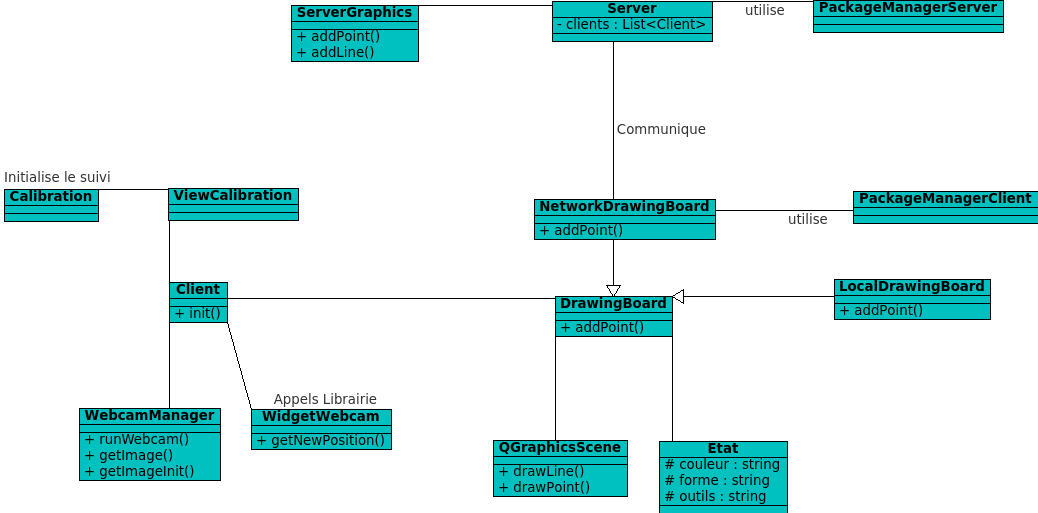
\includegraphics[scale=0.45]{../uml/classes.png}
			\end{center}
		\end{frame}
		
		\subsection{Fonctionnalités}
		\begin{frame}{Fonctionnalités - Outils}
			\begin{center}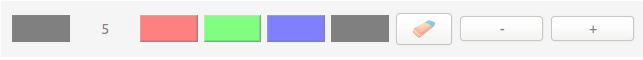
\includegraphics[scale=0.45]{toolbar.png}\end{center}
			\begin{center}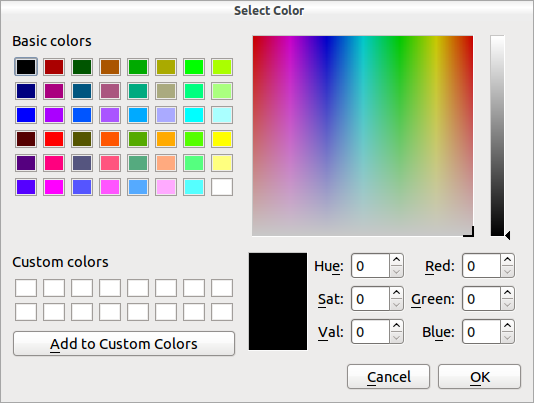
\includegraphics[scale=0.2]{colorpicker.png}\end{center}
			\begin{itemize}
				\item Couleur
				\item Gomme
				\item Taille
				\item Affichage
			\end{itemize}
		\end{frame}
		\begin{frame}{Fonctionnalités - Actions}
			\begin{center}
				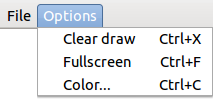
\includegraphics[scale=0.6]{menu.png}\quad
				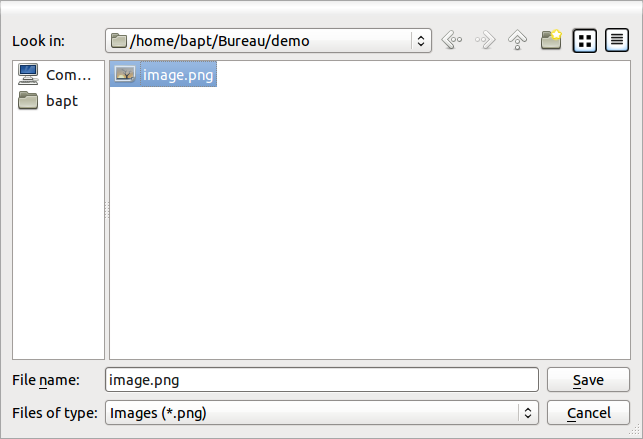
\includegraphics[scale=0.2]{export.png}
			\end{center}
			\begin{itemize}
				\item Sauvegarde du dessin
				\item Vider le tableau
				\item Mode plein écran
			\end{itemize}
		\end{frame}
		
		\subsection{Fonctionnement}
		\begin{frame}{Fonctionnement - Interface intuitive}
			\begin{center}
				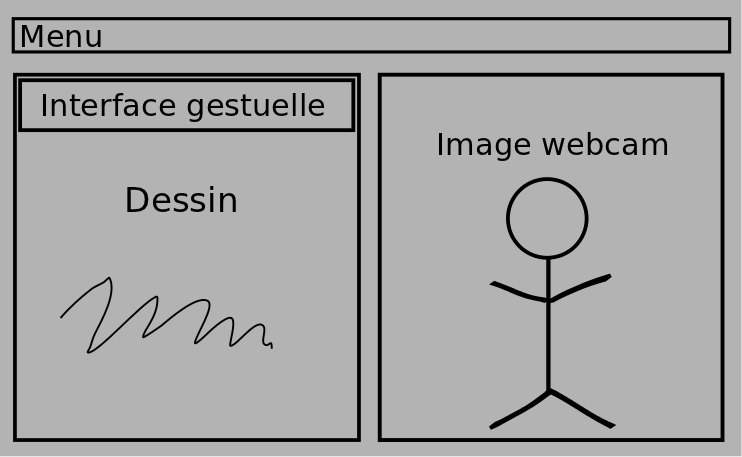
\includegraphics[scale=0.45]{interface.png}
			\end{center}
		\end{frame}
		
		\begin{frame}{Fonctionnement - Etalonnage}
			\begin{block}{Technique}
				\begin{itemize}
					\item Interface "Suivant - Précédent"
					\item Étalonnage obligatoire
				\end{itemize}
			\end{block}
			\begin{block}{Utilisation}
				\begin{enumerate}
					\item Choix webcam / Type de suivi
					\item Sélection de l'objet
					\item Réglage de la tolérance
					\item Choix mode local / réseau
				\end{enumerate}
			\end{block}
			
		\end{frame}
		
		\begin{frame}{Fonctionnement - Local}
			\begin{columns}
				\begin{column}{5cm}
					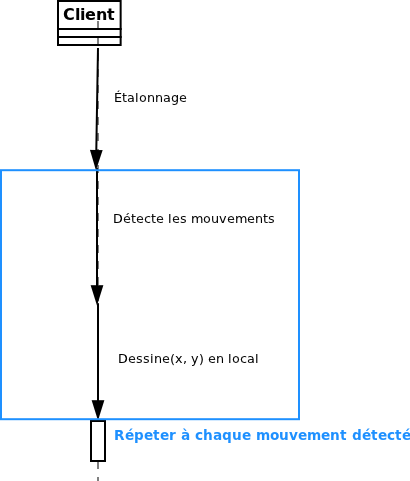
\includegraphics[scale=0.45]{sequence_local.png}
				\end{column}
				\begin{column}{3cm}
					\begin{itemize}
						\item Étalonnage
						\item Détection de l'objet
						\item Dessin
					\end{itemize}
				\end{column}
			\end{columns}
		\end{frame}
		
		\begin{frame}{Fonctionnement - Réseau}
			\begin{columns}
				\begin{column}{9cm}
					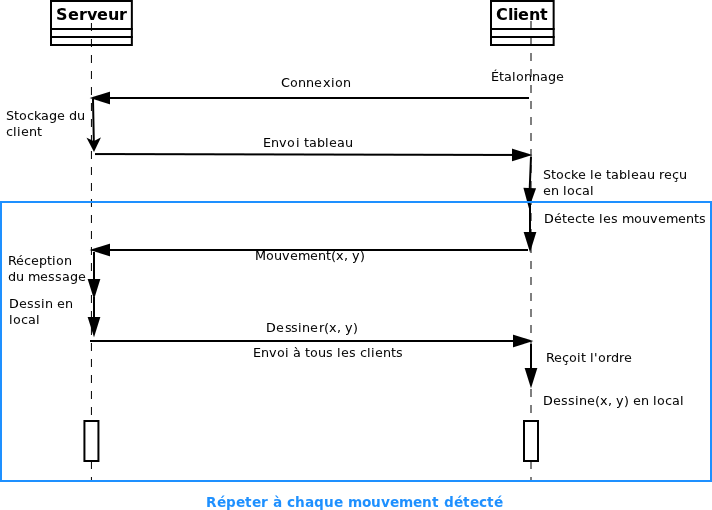
\includegraphics[scale=0.35]{sequence_reseau.png}
				\end{column}
				\begin{column}{5cm}
					\begin{itemize}
						\item Étalonnage
						\item Détection de l'objet
						\item Dessin
					\end{itemize}
				\end{column}
			\end{columns}
		\end{frame}
		
		\subsection{Mise en production}
		\begin{frame}{Mise en production}
			\begin{block}{Pourquoi?}
				\begin{itemize}
					\item Généralement oubliée
					\item Première expérience
					\item Application aboutie
				\end{itemize}
			\end{block}
			\begin{block}{Eléments}
				\begin{itemize}
					\item Traduction
					\item Packaging (.deb)
					\item Documentation
					\item Portabilité
					\item Dépôt accessible
					\item Code propre
				\end{itemize}
			\end{block}
		\end{frame}
		
		\subsection{Ouverture}
		\begin{frame}{Ouverture}
			\begin{itemize}
				\item Amélioration du réseau
				\item Amélioration des performances
				\item Possibilité de relancer l'étalonnage
			\end{itemize}
		\end{frame}

	
      \section{Conclusion}
            \begin{frame}{Conclusion}
                  \begin{exampleblock}{Objectifs atteints}
			\begin{itemize}
                        \item Solution fonctionnelle \\
                        \item Respect du cahier des charges \\
                        \item Découverte (Technologies, gestion de projet...) \\ 
			\end{itemize}
                  \end{exampleblock}
                  \pause
                  \begin{alertblock}{Difficultés}
			\begin{itemize}
                        \item Collaboration : Développement incrémental qui oblige à beaucoup communiquer \\
                        \item Formation : Traitement de l'image, Conception d'architectures \\
                        \item Techniques : Architecture, gestion mémoire\\
			\end{itemize}
                  \end{alertblock}
                  \pause
                  \begin{block}{Ouverture}
			\begin{itemize}
                        \item Diversifier et optimiser les méthodes de suivi \\
                        \item Rajouter des fonctionnalités côté application \\
			\end{itemize}
                  \end{block}
	\end{frame}
      
	\begin{frame}{Sources et bibliographie}
   
		%need tiny{}
		\begin{itemize}
		\item{\url{http://www.sciencedirect.com.www.ezp.biu-montpellier.fr/science/article/pii/S026288561100120X}}
		\item{\url{http://www.irit.fr/recherches/SAMOVA/pageAnalysis.html}}
		\item{\url{http://www.irit.fr/~Philippe.Joly/Teaching/L3SI/ti.html}}
		\item{\url{http://opencv.willowgarage.com/wiki/}}
		\item{\url{code.google.com/p/cvblob/} }
		\end{itemize}
		lien du projet : \url{http://code.google.com/p/dessin-realite-augmentee/}
	\end{frame}

\end{document}
